\documentclass{article}
\usepackage[utf8]{inputenc}
\usepackage{geometry}
\geometry{hmargin=2.5cm,vmargin=2.5cm}
\usepackage{mathtools} %\usepackage{align}
%\usepackage[french]{babel}
\usepackage{graphicx}
\usepackage{amsfonts}

\title{SOD333 - Rapport}
\author{Paul-Antoine Leveilley \& Mila Rocco}
\date{Septembre 2022}

\begin{document}

\maketitle

\begin{center}
Chaque rapport de TP doit faire environ 5 pages.
\end{center}







\newpage
\section{Importance sampling: Codage sur un exemple d'approximation d'une intégrale}

\subsection{Introduction}
On étudie la loi Y = g(X) d'espérance µ définie ci-dessous, où $X \hookrightarrow q$. La fonction de densité q de l'échantillon étudié et la fonction g sont connues et on cherche à estimer l'espérance µ:
$$\mu = \int_0^1 g(x)q(x)dx = \int_0^1 cos(\frac{\pi x}{2})dx\ (=\frac{2}{\pi})$$
Bien que l'on connaisse les deux fonctions, le calcul de l'intégrale de leur produit peut devenir très lourd en temps et en calculs, et il convient donc de trouver une méthode efficace pour l'estimer.

On décide d'étudier l'échantillon $(X_i)_{1\leq i \leq N}$ , qui suit la loi uniforme sur $[0,1]$. On choisira $N=50$ pour l'étude empirique du problème.

 \subsection{Application "brute" de la Méthode de Monte Carlo}
Dans un premier temps, on choisit d'estimer µ avec la méthode brute de Monte Carlo. On choisit l'estimateur: $$\hat{\mu}_N = \frac{1}{N} \sum_{i=1}^N g(X_i)$$

- Calculer la variance théorique\\
\begin{align*} 
  Var(\hat{\mu}_N) &= \frac1{N^2} \sum_{i=1}^N Var(g(X_i))\\ 
  &= \frac1{N^2}\times N Var(cos(\frac{\pi X}2)) \\ 
  &= \frac1{N} \left ( \int_0^1 cos^2(\frac{\pi x}2)dx - \left ( \int_0^1 cos(\frac{\pi x}2)dx \right )^2 \right )\\
  &= \frac1{N} \left ( \int_0^1 \frac{1+cos(\pi x)}{2}dx - 
   \frac4{\pi^2} \right )\\
  &= \frac1{N} \left ( \frac{1}{2} - 
   \frac4{\pi^2} \right )\\
  &\approx \frac{9,47.10^{-2}}{N} \approx 1,89.10^{-3}
\end{align*}

- Estimer empiriquement la variance\\
On tire un échantillon de $NbMC=1000$ tirages. On obtient alors une variance empirique de $1,84.10^{-3}$, qui est très proche du calcul théorique, comme attendu.

On vérifie maintenant que le TCL est cohérent. On observe Figure~\ref{TP1_MC_TCL} la comparaison du TCL appliqué aux erreurs relatives de nos échantillons, avec la gaussienne centrée réduite. Les résultats sont donc bien cohérents avec nos calculs théoriques de moyenne et de variance.

\begin{figure}[ht]
\centering
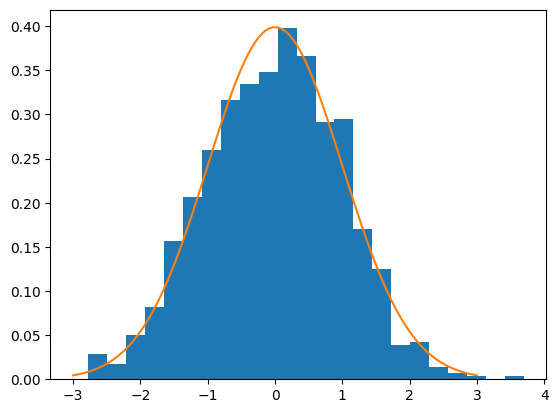
\includegraphics[width=0.4\textwidth]{TP1/MC_brute_TCL.png}
\caption{résultat du TCL}
\label{TP1_MC_TCL}
\end{figure}



\subsection{Echantillonage pondéré}
On effectue dans le calcul de µ le changement de probabilité suivant:
$$ \mu = \int_0^1 g(x)q(x)dx = \int_0^1 \frac{g(x)q(x)}{\Tilde{q}(x)} \Tilde{q}(x) dx $$

Cela revient maintenant à étudier $Y=\frac{g(Z)q(Z)}{\Tilde{q}(Z)}$, où la variable aléatoire Z est de densité $\Tilde{q}$. On appelle $\Tilde{q}$ la "Fonction d'Importance". L'objectif étant d'estimer le produit de g et q, on voudrait estimer $\Tilde{q}$ pour qu'il soit le plus proche possible de la loi de probabilité $p(x) = \frac{g(x)q(x)}{\int_{[0,1]} g(u)q(u)du}$.

La méthode du rejet nous donne que si
\begin{itemize}
 \item $X \hookrightarrow q,\ U \hookrightarrow U([0,1])$ et $\forall x, g(x) \leq C$ (dans notre cas, C = 1)
 \item Si $g(X) \geq CU$, poser $Z=X$
\end{itemize}

Alors, $Z \hookrightarrow p $\\

On génère un toujours l'échantillon $(X_i)_{1\leq i \leq N}$ suivant maintenant la loi uniforme de densité q. On génère ensuite Z par la méthode du rejet, et l'on peut ainsi estimer µ comme suit: 
$$ \hat{\mu}_N = \frac1{N} \sum_{i=1}^N g(X_i)\frac{q(X_i)}{\Tilde{q}(X_i)}\ \overset{p.s.}{\longrightarrow}\ \mu $$

- Chercher une bonne FI (idée: DL au voisinage de 0)  \\
Pour choisir $\Tilde{q}$, on approxime la fonction g par son développement à l'ordre 2 en 0. Rappelons le développement limité en 0 de la fonction cosinus: 
$ cos(x) = 1 - \frac{x^2}{2} + o(x^2) $.
On prend donc pour Fonction d'Importance: 
$$\Tilde{q}_1(x):= 1 - \frac{\pi^2}{8} x^2 $$
Il est important de prendre en compte le fait que $\Tilde{q}$ ne doit pas s'annuler si gq ne s'annule pas. Le DL doit donc être corrigé pour que $\Tilde{q}$ ne devienne pas négatif en $x=1$. En $x=1$, la fonction précédente vaut $\delta = 1 - \frac{\pi^2}{8} < 0$, donc on soustrait $\delta$ à $\Tilde{q}_1$ pour obtenir notre nouvelle fonction d'importance :
$$\Tilde{q}_2(x):= \frac{\pi^2}{8}(1 - x^2) $$

- Calcul de la variance théorique
\begin{align*} 
  Var(\hat{\mu}_N) &= \frac1{N^2} \sum_{i=1}^N Var \left ( g(X_i)\frac{q(X_i)}{\Tilde{q}(X_i)}\right)\\ 
  &= \frac1{N} \left ( \int_0^1 \left (\frac{g(x)q(x)}{\Tilde{q}(x)} \right )^2 \Tilde{q}(x) dx  - \left ( \int_0^1 \frac{g(x)q(x)}{\Tilde{q}(x)} \Tilde{q}(x) dx \right )^2 \right )\\
  &= \frac1{N} \left ( \int_0^1 \frac{g^2(x)q^2(x)}{\Tilde{q}(x)} dx  - \left ( \int_0^1 g(x)q(x) dx \right )^2 \right )\\
  &= \frac1{N} \left ( \int_0^1 \frac{cos^2(\frac{\pi x}2)}{\frac{\pi^2}{8} (1 -  x^2)} dx   - \mu^2 \right )\\
  &\approx 1,98.10^{-5}\\
\end{align*}

- Calcul de la probabilité d'acceptation théorique:
$$P_a = \frac1C \int_0^1 g(x)q(x)dx 
= \int_0^1 cos(\frac{\pi x}{2})dx 
=\frac{2}{\pi} 
\approx 0,637$$

\textbf{Application numérique (TP):}\\
Les Figures~\ref{TP1_IS_DL} et~\ref{TP1_IS_TCL} nous montrent l'étude des deux FI $\Tilde{q}_1$ et $\Tilde{q}_2$ définies précédemment.

\begin{figure}[ht]
\centering
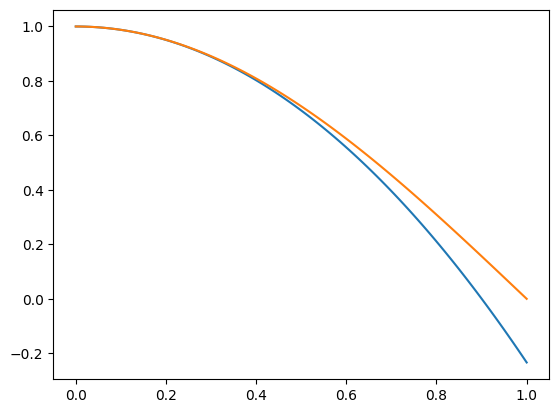
\includegraphics[width=0.4\textwidth]{TP1/DL_ordre2_g.png}
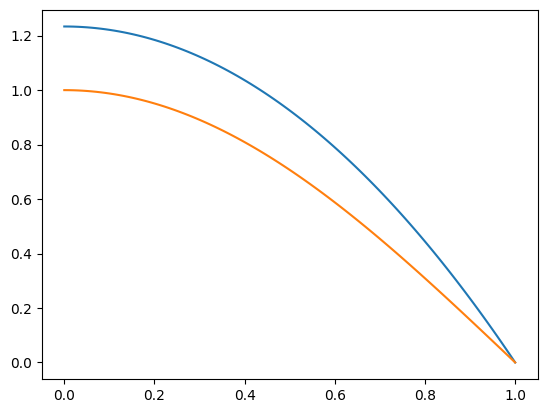
\includegraphics[width=0.4\textwidth]{TP1/DL_ordre2_corrige.png}
\caption{représentation des fonctions gq (en orange) et $\Tilde{q}$ (en bleu): à gauche $\Tilde{q}_1$, à droite $\Tilde{q}_2$}
\label{TP1_IS_DL}
\end{figure}

\begin{figure}[ht]
\centering
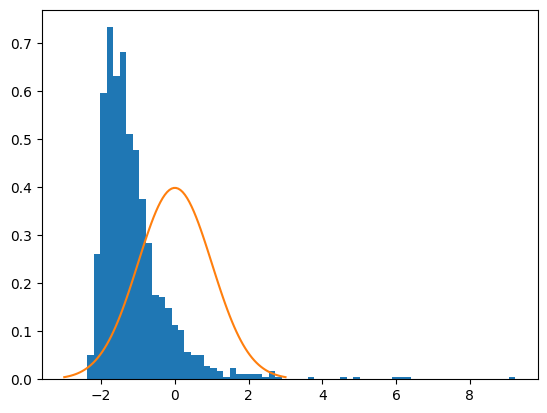
\includegraphics[width=0.4\textwidth]{TP1/IS_TCL_DL_ordre2.png}
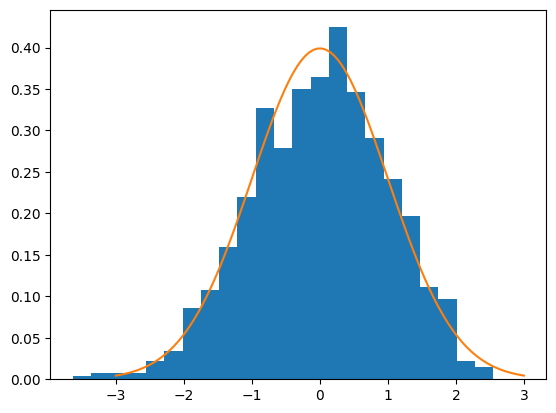
\includegraphics[width=0.4\textwidth]{TP1/IS_TCL_DL_ordre2_corrige.png}
\caption{TCL appliqués respectivement à $\Tilde{q}_1$ (à gauche) et $\Tilde{q}_2$ (à droite)}
\label{TP1_IS_TCL}
\end{figure}

Les résultats du TCL appliqués aux échantillons produits mettent ici en valeur l'importance d'avoir une fonction d'importance du même signe que gq, mais aussi que notre développement limité en 0 corrigé de gq $\Tilde{q}_2$  semble être une bonne approximation pour notre problème. On obtient en effet une variance empirique $Var(\hat{\mu}_N) = 2,11.10^{-5} $ et une probabilité d'acceptation $P_a = 0,669$.



\subsection{Conclusion}
On cherche maintenant à comparer les deux méthodes précédemment appliquées.

- Comparer le rapport des variances des 2 méthodes (théoriquement et par simulations)\\
% $$\frac{variance\ th\'eorique (Monte\ Carlo)}{variance\ th\'eorique (Importance\ Sampling)} = \frac{1,89.10^{-3}}{1,97.10^{-5}} \approx 95,6 $$
% $$\frac{variance\ empirique (Monte\ Carlo)}{variance\ empirique (Importance\ Sampling)} = \frac{1,84.10^{-3}}{2,11.10^{-5}} \approx 83,7 $$
On en conclue donc que la méthode d'Importance Sampling est bien meilleure.\\

- Valider par simulations les TCL pour les 2 méthodes en comparant la loi théorique (loi normale) à la loi empirique (histogramme)\\
Les figures~\ref{TP1_MC_TCL} et~\ref{TP1_IS_TCL} nous prouvent que la distribution de l'erreur faite par nos estimateurs suivent une gaussienne centrée réduite, donc valident nos approximations de µ.\\

- Comparer les budgets pour chaque méthode\\
\textbf{TO DO}\\

- Calculer la variance de l’estimateur en prenant la FI optimale\\
Lorsqu'on choisit $\Tilde{q}=gq/ \int g(x)q(x)dx$, on obtient une variance empirique nulle pour la méthode d'Importance Sampling et une estimation de la probabilité d'acceptation d'environ 0,64. La variance théorique vaut quant à elle $P_a(theo)=-2,22.10^{-18}\approx 0$ (erreur d'arrondi de l'ordinateur) et la Probabilité d'acceptation théorique $=0.637$.\\










\newpage
\section{Filtre de Kalman: Poursuite d'un mobile en mouvement rectiligne uniforme bruité}
\subsection{Introduction}
Dans ce TP, nous allons simuler la trajectoire d'un mobile, et tenter de retrouver ces valeurs grâce à des observations que nous aurons de sa trajectoire.

On considère l'état à l'instant t $X_t$ où t varie entre 0 et T, et sa mesure $Y_t$
\[ X_t = \left (
   \begin{array}{c}
      x_t \\
      y_t \\
      \Dot{x_t} \\
      \Dot{y_t} \\
   \end{array} \right )
   ,\ Y_t = \left (
   \begin{array}{c}
      x_t \\
      y_t \\
   \end{array} \right )
   ,\ W_t = \left (
   \begin{array}{c}
      w_t^1 \\
      w_t^2 \\
   \end{array} \right )
\]

équation de la dynamique : 
\[ m \left (
   \begin{array}{c}
      \ddot{x_t} \\
      \ddot{y_t} \\
   \end{array} \right )
   = \left (
   \begin{array}{c}
      w_k^1 \\
      w_k^2 \\
   \end{array} \right )\ 
   \forall t \in [t_k, t_{k+1}]
\]

On fixe $m=1$ et on obtient l'équation d'état suivante :
\[ X_n = \left ( 
   \begin{array}{cccc} %Fn
      1 & 0 & \delta t & 0 \\
      0 & 1 & 0 & \delta t \\
      0 & 0 & 1 & 0 \\
      0 & 0 & 0 & 1 \\
   \end{array} \right )
   \left ( 
   \begin{array}{cccc} %Xn-1
      x_{t_{n-1}} \\
      y_{t_{n-1}} \\
      \Dot{x}_{t_{n-1}} \\
      \Dot{y}_{t_{n-1}} \\
   \end{array} \right )
   + \left (
   \begin{array}{cc}
      \frac{c(\delta t)^2}{2m} & 0 \\
      0 & \frac{c(\delta t)^2}{2m} \\
      \frac{c\delta t}{m} & 0 \\
      0 & \frac{c\delta t}{m} \\
   \end{array} \right )
   \left (
   \begin{array}{c}
      w_n^1 \\
      w_n^2 \\
   \end{array} \right )
   = F X_{n-1} + G W_n
\]

Condition initiale: 
\[ m_0 = \mathbb{E}[X_0] = \left (
   \begin{array}{c}
      5000\ m \\
      5000\ m \\
      -20\ m/s \\
      20\ m/s \\
   \end{array} \right )
   ,\ P_0 = \left (
   \begin{array}{cccc}
      (2000\ m)^2 & 0 & 0 & 0 \\
      0 & (2000\ m)^2 & 0 & 0 \\
      0 & 0 & (5\ m/s)^2 & 0 \\
      0 & 0 & 0 & (5\ m/s)^2 \\
   \end{array} \right )
\]

Constantes du problème:
$$ \left\{
   \begin{array}{l}
      \delta t = 1\ seconde\\
      T = N \delta t = 200\ s \\
      c = 2\ m/s^2 \\
   \end{array} \right .$$

\begin{figure}[ht]
\centering
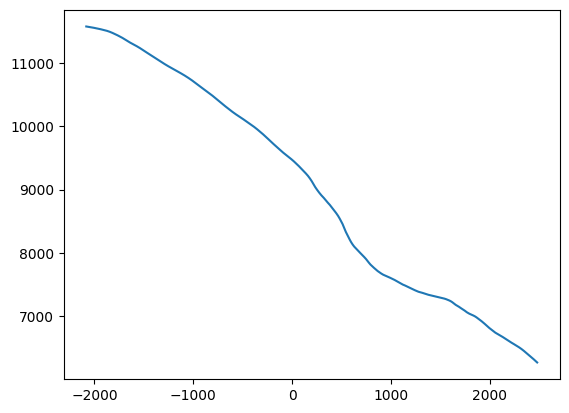
\includegraphics[width=0.4\textwidth]{TP2/position_réelle.png}
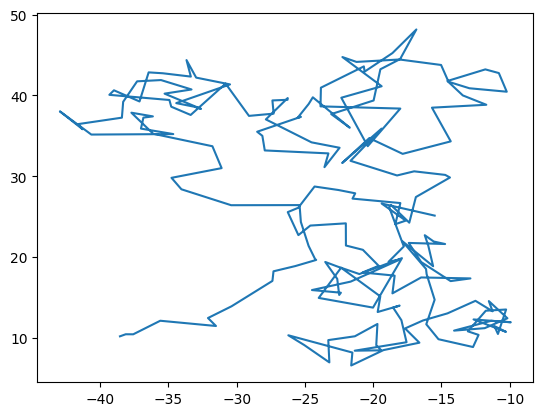
\includegraphics[width=0.4\textwidth]{TP2/vitesse_reelle.png}
\caption{Trajectoire et vitesse associée, que l'on cherche à retrouver}
\label{TP2_pos_vit}
\end{figure}

\subsection{Titre intermédiaire}
\subsection{Conclusion}


\newpage

\section{TP3 : Borne de Cramer Rao.}
\subsection{Introduction}
\subsubsection{Formulation du problème}

Dans ce TP, on se propose de calculer une borne de Cramer Rao pour un problème de filtrage. Le cadre général est le suivant.
On se donne un système  $(X_{k})_{k\geq 0}$ sujet à une certaine dynamique,
ainsi qu'une série de mesures bruitées $(y_{k})_{k \geq 0}$ (bruit gaussien de variance $\sigma_{k}^{2}$) : 
\[\left\{\begin{array}{ll}
   X_{k+1} = \phi(k,k+1)X_{k} \\
   y_{k}=h_{k}(X_{k})+\epsilon_{k}
\end{array}\right. \]

Avec $X_{0} \sim  \mathcal{N} (X_{\nu},P_{0})$. On peut montrer que la matrice d'information ralative à l'instant $k$ vérifie
la relation de récurence suivante : 

\[ J_{k} = \frac{1}{\sigma_{k}}\left(\frac{\partial h_{k}}{\partial X_{k}}\right)\left(\frac{\partial h_{k}}{\partial X_{k}}\right)^{T}+\left(\frac{\partial X_{k-1}}{\partial X_{k}}\right)^{T}J_{k-1}\left(\frac{\partial X_{k-1}}{\partial X_{k}}\right)\]

Avec $J_{0}=P_{0}^{-1}$ et $\phi(k,k+1)=\frac{\partial X_{k+1}}{\partial X_{k}}$.
La borne de Cramer Rao à l'instant $k$ est alors égale à l'inverse de la matrice d'information : 
\[BCR_{k}= J_{k}^{-1}\]

Nous étudions le système suivant : un bateau émetteur de bruit se déplace dans le plan de manière rectiligne uniforme. 
Un bateau observateur mesure la direction d'ou lui parvient le bruit, plus précisément, il mesure l'angle $\theta_{k}$ que fait cette direction avec l'horizontale, ce toute les secondes pendant 100s. Le bateau observateur se déplace également en ligne droite à vitesse constante.
Si l'état de l'émeteur est donné par sa position et sa vitesse : $X_{k} = (x_{k},y_{k},\dot{x}_{k},\dot{y}_{k})$, sa matrice de transition est :
\[\phi(k,k+1) = \phi =  \begin{pmatrix}
  1 & 0 & T & 0 \\
  0 & 1 & 0 & T \\
  0 & 0 & 1 & 0 \\
  0 & 0 & 0 & 1 
  \end{pmatrix}\]

Pour pouvoir discriminer entre différentes
trajectoires possibles, le bateau doit virer de bord à un certain moment. Si ça n'est pas le cas, on peut vérifier que des trajectoires différentes peuvent donner lieu à des mesures d'angle identiques.
Pour simplifier l'étude, on suppose que le bateau vire de bord toujours au même moment : au milieu du trajet. Le bateau observateur choisit l'angle $\varphi $ duquel il tourne. Chaque choix de $\varphi$ 
conduit à une précision différente de l'estimation de la trajectoire  de l'émeteur.
La question est donc la suivante : quel choix de $\varphi$ est le meilleur pour estimer la trajectoire de l'émeteur?
\\
Pour répondre à cette question, nous allons simuler la dynamique de l'éméteur et de l'observateur. Grâce à ces dynamiques, nous allons
calculer le gradient de la fonction d'observation et nous allons en déduire la matrice d'information.
Dans notre cas, la fonction d'observation est l'angle que fait la direction d'observation avec l'horizontale. 
En terme de l'abscisse et de l'ordonnée de l'éméteur et de l'observateur, cette fonction s'écrit : 
\[\theta_{k} = h_{k}(X_{k})=\arctan \left(\frac{y_{k}-y_{k}^{o}}{x_{k}-x_{k}^{o}}\right)\]

En inversant la matrice d'observation, on obtiendra la borne de Cramer Rao, sous forme d'une matrice carrée d'ordre 4.
On cherchera ensuite la valeur de $\varphi$ qui minimise le critère : $\sqrt{\sigma_{x_{n}}^{2}+\sigma_{y_{n}}^{2}}$

\subsubsection{Calcul du gradient de $h_{k}$ par rapport à $X_{k}$}
Déjà, on voit facilement que : 
\[\frac{\partial h_{k}}{\partial \dot{x}_{k}} = 0 \] et :
\[\frac{\partial h_{k}}{\partial \dot{y}_{k}} = 0 \]
Ensuite, par le calcul, on a que : 
\[\frac{\partial h_{k}}{\partial x_{k}}=\frac{y_{k}^{o}-y_{k}}{\left(x_{k}-x_{k}^{o}\right)^{2}\left(1+\left(\frac{y_{k}-y_{k}^{o}}{x_{k}-x_{k}^{o}}\right)^{2}\right)}\]
et :

\[\frac{\partial h_{k}}{\partial y_{k}}= \frac{1}{\left(x_{k}-x_{k}^{o}\right)\left(1+\left( \frac{y_{k}-y_{k}^{o}}{x_{k}-x_{k}^{o}}  \right)^{2}\right)}\]
\subsection{Simulations des dynamiques de l'observateur et de l'émetteur}
Nous avons simulé la dynamique du système pour différents changements de cap de l'observateur, avec les paramètres du tableau \ref{paramètres}.
 Nous obtenons les tracés de la figure \ref{trajectoire}


\begin{figure}[h!]
  \centering
  \caption{Paramètres pour la simulation}
  \label{paramètres}
  \begin{tabular}{|*{11}{c|}}
    \hline Horizon temporel & $T = 1$ \\
    \hline Nombre de mesures  & $N=100$ \\
    \hline Ecart type du bruit & $\sigma_{k}=1^{\circ}$\\
    \hline Vitesse de l'observateur & $V_{o}=10 m.s^{-2}$\\
    \hline Position initiale de l'observateur &  $(x_{0}^{o},y_{0}^{o})=(0,0)$ m\\
    \hline Vitesse de l'émetteur & $V_{e} = 5 m.s^{-2}$\\
    \hline Cap de l'émetteur & $\alpha =-20^{\circ}$\\
    \hline Position initiale de l'émetteur & $(x_{0},y_{0})=(2000,2000)$\\
    \hline Incertitude initiale sur la position de l'émetteur & $P_{0}=diag(1000,1000,10,10)^{2}$\\
    \hline
  \end{tabular}
\end{figure}


 \begin{figure}[h!]
  \centering
  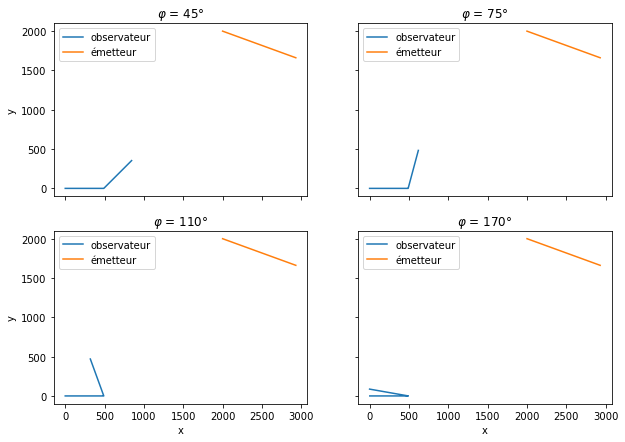
\includegraphics[width = 15cm]{TP3/trajectoires.png}
  \label{trajectoire}
  \caption{Trajectoires de l'émetteur et de l'observateur pour différentes valeurs de l'angle $\varphi$}
\end{figure}

Grâce à ces dynamiques, nous sommes capables de calculer la Borne de Cramer Rao associée à cet estimateur de la position de l'émetteur. 
Nous présentons ces résultat en figure \ref{cramerrao}. 

\begin{figure}[h!]
  \centering
  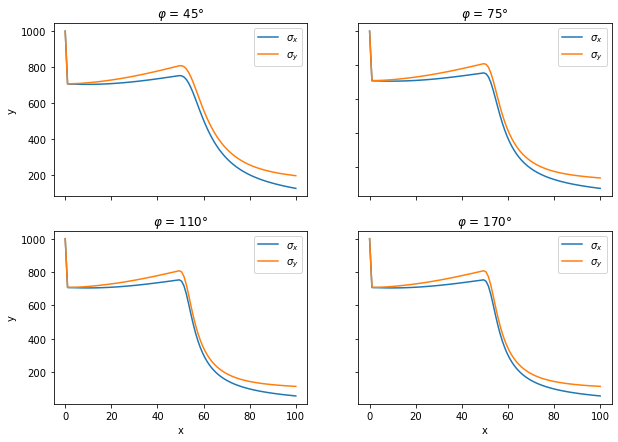
\includegraphics[width = 15cm]{TP3/cramer rao.png}
  \caption{Borne de Cramer Rao pour l'abscisse et l'ordonnée de la position de l'émetteur au cours du temps, pour différentes valeurs de $\varphi$}
  \label{cramerrao}
\end{figure}

\subsection{Optimisation de la valeur de $\varphi$}
Pour trouver la valeur de $\varphi$ optimale, nous avons simplement testé toutes les valeurs entre $0^{\circ}$ et $360^{\circ}$, avec un pas de 
$1^{\circ}$. Nous avons trouvé une valeur optimale de $\varphi = 109^{\circ}$, ce qui correspond à la trajectoire représentée en figure
\ref{optimale}. La borne de Cramer Rao associée est représentée en figure \ref{crameropti}. Le critère associé est un écart type sur la position de 128m.
\begin{figure}
  \centering
  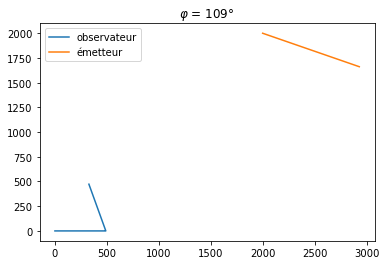
\includegraphics[width = 10 cm]{TP3/trajopti.png}
  \label{optimale}
  \caption{Trajectoire optimale pour l'observateur}
\end{figure}

\begin{figure}
  \centering
  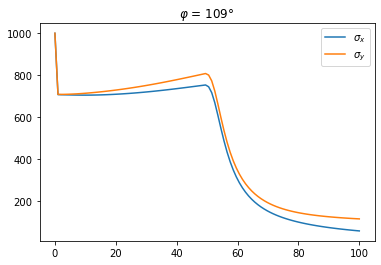
\includegraphics[width = 10 cm]{TP3/crameropti.png}
  \label{crameropti}
  \caption{Borne de Cramer Rao pour la trajectoire optimale}
\end{figure}

\subsection{Conclusion}
En conclusion, ce TP nous aura permis de voir comment la Borne de Cramer Rao permet de réaliser le choix d'une stratégie pour 
optimiser la précision sur l'estimation de état d'un système, grâce à la seule connaissance d'un modèle à priori.

\newpage

\section{TP4: titre du TP}
\subsection{Introduction}

\subsection{Titre intermédiaire}

\subsection{Conclusion}


\end{document}
